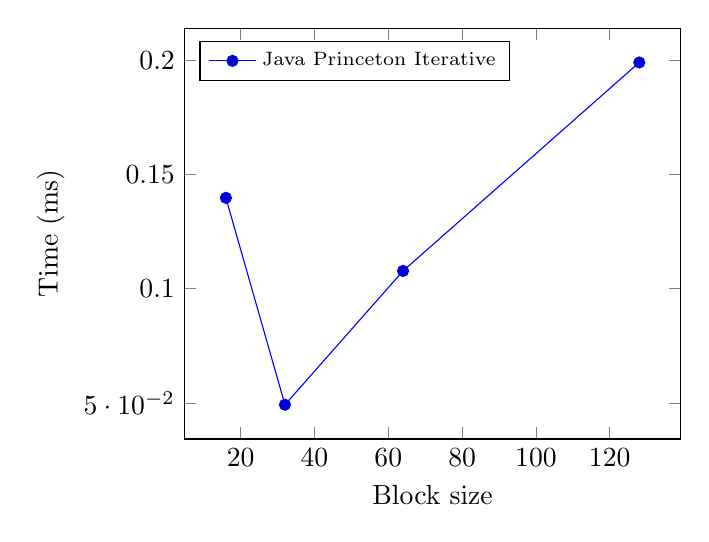
\begin{tikzpicture}
\begin{axis}[xlabel={Block size},ylabel={Time (ms)},width=0.65\linewidth,legend pos=north west,scaled y ticks = false,legend cell align=left,legend style={font=\scriptsize}]
\addplot coordinates {
(16, 0.1398)
(32, 0.0492)
(64, 0.1078)
(128, 0.1991)
};
\legend{Java Princeton Iterative}
\end{axis}
\end{tikzpicture}
